This plugin implements a vacuum tube simulation that generates distortions.

This simulation applies a qualitative model of vacuum tubes. It consists of two stages: First, the output characteristics of a triode vacuum tube are simulated:
%
\begin{equation}
  I(x) = \max\{x+x_0,0\}^{\frac32}
\end{equation}
%
Here $x$ corresponds to the grid voltage, $x_0$ to the grid bias voltage and $I$ to the anode current. In this qualitative model, the anode voltage is not explicitly considered.
%
The second stage simulates the overdrive:
\begin{equation}
  \hat I(x) = \frac{I(x)}{I(x)+s}
\end{equation}
with the saturation parameter $s$, and the limited anode current $\hat I$.
%
The offset of the simulation output signal is then corrected, and a pre-gain $p_i$ and a post-gain $p_o$ is applied:
\begin{equation}
  y(x) = g_o \cdot \left(\hat I \left(g_i \cdot x \right) - \hat I\left(x_0\right)\right)
\end{equation}
%
The resulting input-output characteristics, sine waveform and distortion spectrum is shown in Figure \ref{fig:tubesim}.

\begin{figure}[htb]
  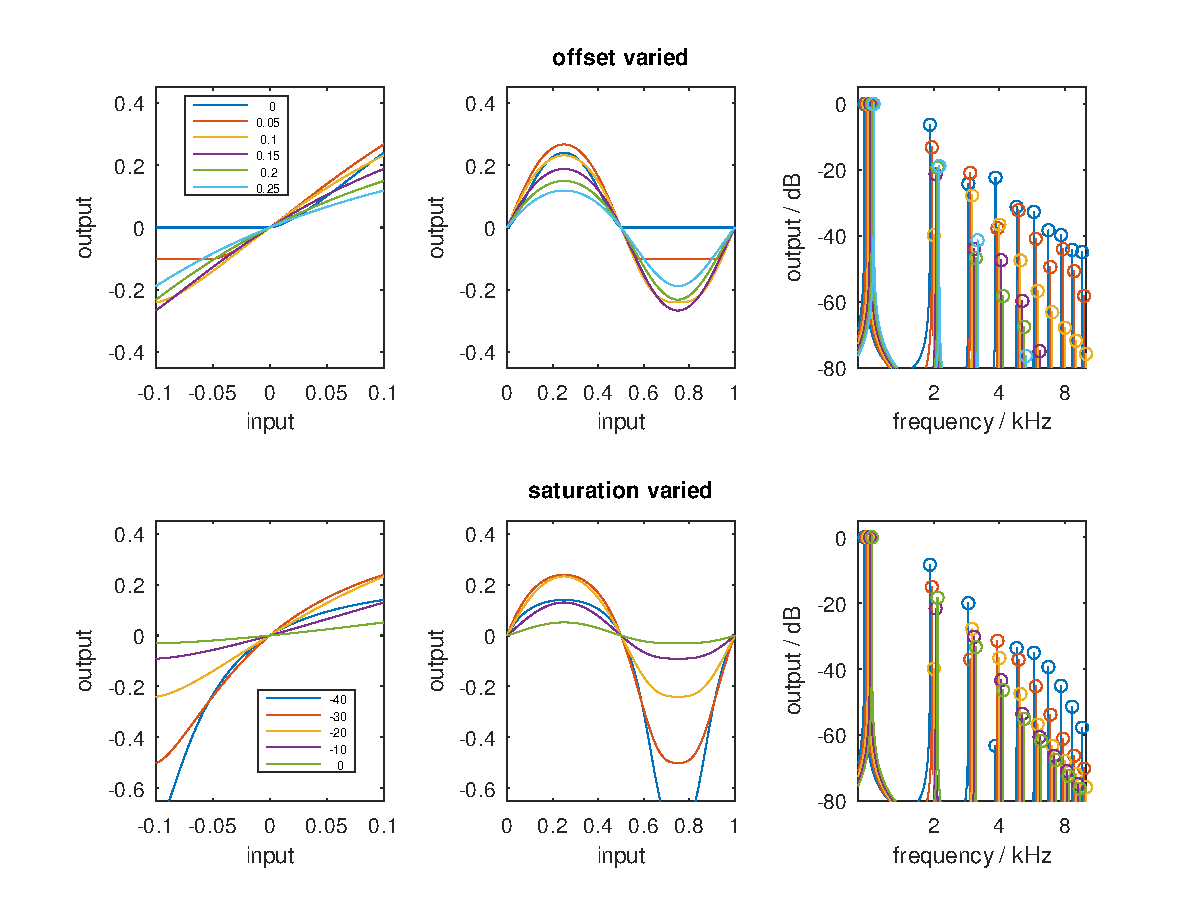
\includegraphics[width=\textwidth]{tubesim.pdf}
  \caption{Input-output characteristics (left panel), sine waveform (middle panel) and distortion spectrum (right panel) of the tube simulation for various offset parameters $x_0$ (upper row) and saturation values $20\log10(s)$ (lower row).}\label{fig:tubesim}
\end{figure}

\definecolor{shadecolor}{RGB}{255,230,204}\begin{snugshade}
{\footnotesize
\label{attrtab:tubesim}
Attributes of element {\bf tubesim}\nopagebreak

\begin{tabularx}{\textwidth}{l>{\raggedright}XX}
\hline
name & description (type, unit) & def.\\
\hline
\hline
\indattr{bypass} & Bypass plugin (bool) & false\\
\hline
\indattr{offset} & Input offset $x\_0$ (float) & 0.5\\
\hline
\indattr{postgain} & Post-gain $g\_o$ (float, dB) & 0\\
\hline
\indattr{pregain} & Pre-gain $g\_i$ (float, dB) & 0\\
\hline
\indattr{saturation} & Saturation parameter $s$ (float, dB) & -6.0206\\
\hline
\indattr{wet} & Wet (1) - dry (0) mixture gain (float) & 1\\
\hline
\end{tabularx}
}
\end{snugshade}

